\section{Desarrollo experimental, comparación de modelos y resultados}
\label{sec:desarrollo_comp_results}

\subsection{Planteamiento experimental y justificación}
\label{sec:planteamiento_experimental}

El presente capítulo recoge el desarrollo experimental llevado a cabo para validar la hipótesis principal del Trabajo Fin de Máster: que el uso de una arquitectura basada en \textit{Transformers} con mecanismos de atención espacial, como \textit{Trafficformer}, permite mejorar la capacidad predictiva respecto a modelos tradicionales como un perceptrón multicapa (\textit{MLP}) en el contexto de predicción de aforos de tráfico.

Para ello, se ha diseñado una estrategia de evaluación comparativa entre modelos, aplicándolos sobre tres fuentes de datos independientes que recogen información de tráfico rodado en la provincia de Bizkaia. Cada fuente representa una infraestructura y cobertura distintas, lo que permite evaluar el comportamiento de los modelos bajo distintos escenarios y estructuras de datos.

\subsubsection*{Propósito e hipótesis del experimento}

El objetivo del experimento es doble:

\begin{enumerate}
	\item \textbf{Evaluar el rendimiento comparativo} de dos modelos de predicción de tráfico: un modelo base (MLP) y un modelo avanzado (Trafficformer), bajo las mismas condiciones de entrenamiento y sobre las tres fuentes de datos.
	\item \textbf{Analizar el impacto del diseño de arquitectura y la configuración de parámetros} sobre el rendimiento predictivo en escenarios heterogéneos, valorando especialmente la aportación del mecanismo de atención espacial.
\end{enumerate}

La hipótesis de partida es que el modelo \textit{Trafficformer}, al integrar mecanismos de atención multi-cabeza junto con máscaras espaciales basadas en OpenStreetMap, será capaz de capturar relaciones espaciales y temporales complejas entre sensores de tráfico, lo que se traducirá en mejores métricas de error respecto a una MLP.

Antes de abordar las particularidades técnicas de cada arquitectura en apartados posteriores, en la Tabla~\ref{tab:mlp_vs_trafficformer} se presenta una comparación conceptual entre los dos modelos evaluados: un perceptrón multicapa clásico (MLP) y el modelo propuesto basado en atención (Trafficformer).

\begin{table}[H]
	\centering
	\caption{Comparación conceptual entre los modelos MLP y Trafficformer}
	\label{tab:mlp_vs_trafficformer}
	\begin{tabularx}{\textwidth}{lXX}
		\toprule
		\textbf{Característica} & \textbf{MLP (modelo base)} & \textbf{Trafficformer (modelo avanzado)} \\
		\midrule
		Tipo de arquitectura & Perceptrón multicapa clásico & Transformer con atención espacial enmascarada \\
		Entrada esperada & Tensor vectorizado por muestra & Tensor estructurado por sensor y ventana temporal \\
		Captura de relaciones espaciales & No & Sí, mediante mecanismos de atención enmascarada \\
		Robustez ante ruido estructural & Limitada & Alta, gracias al diseño atencional con máscara espacial \\
		Interpretabilidad & Alta (modelo simple) & Media (visualización de atención posible, pero más compleja) \\
		Tiempo de entrenamiento & Bajo & Elevado \\
		Requisitos computacionales & Moderados & Altos (uso de GPU y optimización de memoria) \\
		\bottomrule
	\end{tabularx}
\end{table}

\subsubsection*{Estrategia comparativa}

La estrategia consiste en:

\begin{itemize}
	\item Entrenar ambos modelos (MLP y Trafficformer) sobre cada \texttt{source\_id}, utilizando combinaciones diversas de hiperparámetros.
	\item Evaluar los resultados sobre un conjunto de test independiente, tras aplicar \textit{early stopping} sobre validación.
	\item Seleccionar el mejor modelo para cada combinación (source\_id, modelo), basándose en las métricas MAE, RMSE y $R^2$.
	\item Realizar comparativas cruzadas entre MLP y Trafficformer dentro de cada source, y globalmente.
\end{itemize}

Este enfoque permite no solo identificar el modelo óptimo por entorno de datos, sino también validar si la mejora obtenida por el modelo basado en atención es consistente y significativa. En apartados posteriores se detallarán las configuraciones evaluadas, el entorno de experimentación y los resultados obtenidos.

\subsection{Entorno de desarrollo y reproducibilidad}
\label{sec:entorno_reproducibilidad}

Este apartado describe el conjunto de herramientas, tecnologías y decisiones que han permitido asegurar la trazabilidad, reproducibilidad y escalabilidad de los experimentos realizados en este trabajo. Se detallan tanto el entorno software empleado como las herramientas de seguimiento, exportación y despliegue previstas.

\subsubsection*{Entorno de desarrollo y gestión del proyecto}

La experimentación ha sido desarrollada en un proyecto Python estructurado bajo el paquete \texttt{trafficformer-bizkaia}, gestionado mediante el gestor de dependencias \texttt{uv}. Este gestor ha demostrado ser una alternativa eficiente y moderna a sistemas tradicionales como \texttt{pip} o \texttt{poetry}, permitiendo la instalación aislada de entornos y una resolución rápida de paquetes.

El conjunto de dependencias empleadas en el desarrollo del proyecto se encuentra detallado en el archivo \texttt{pyproject.toml}. A continuación, se enumeran las principales librerías utilizadas, acompañadas de una breve descripción de su función dentro del flujo de trabajo:

\begin{itemize}
	\item \textbf{numpy} y \textbf{pandas}: Bibliotecas fundamentales para la manipulación y análisis eficiente de datos numéricos y estructurados en Python. Permiten operaciones vectorizadas, gestión de grandes volúmenes de datos y transformaciones avanzadas, esenciales en el preprocesamiento y análisis exploratorio.
	
	\item \textbf{scikit-learn}: Conjunto de herramientas de aprendizaje automático clásico, utilizado para la normalización de datos, particionado de conjuntos y evaluación mediante métricas estándar, así como para el desarrollo y comparación de modelos base.
	
	\item \textbf{torch}, \textbf{torchvision} y \textbf{torchaudio}: Paquete principal de PyTorch, framework de referencia para el desarrollo y entrenamiento de modelos de deep learning. Permiten la implementación eficiente de arquitecturas neuronales avanzadas, como Transformers, así como la integración con módulos especializados para visión y audio.
	
	\item \textbf{wandb}: Plataforma para el seguimiento, registro y visualización de experimentos de aprendizaje automático, facilitando la comparación reproducible de resultados y el ajuste de hiperparámetros.
	
	\item \textbf{matplotlib} y \textbf{seaborn}: Herramientas de visualización de datos que permiten generar gráficos y representaciones visuales de resultados, métricas de entrenamiento y análisis exploratorio.
	
	\item \textbf{pymongo}: Cliente de Python para la base de datos MongoDB, utilizado para la gestión y consulta eficiente de grandes volúmenes de datos históricos de tráfico y meteorología.
	
	\item \textbf{geopy} y \textbf{folium}: Librerías para el procesamiento y visualización de datos geoespaciales. Permiten la geolocalización, el cálculo de distancias y la creación de mapas interactivos con información relevante sobre la red viaria.
	
	\item \textbf{onnx}, \textbf{onnxscript} y \textbf{onnxruntime}: Conjunto de herramientas para la exportación y ejecución de modelos en formato ONNX, facilitando la interoperabilidad y el despliegue de modelos en entornos heterogéneos o en producción.
	
	\item \textbf{osmnx}: Biblioteca para la descarga y análisis de datos de redes viarias desde OpenStreetMap, utilizada para la construcción de grafos topológicos que representan la infraestructura de carreteras de Bizkaia.
	
	\item \textbf{tabulate}: Herramienta auxiliar para la generación de tablas en formato texto, útil para la presentación estructurada de resultados y métricas.
	
	\item \textbf{python-dotenv}: Permite la gestión de variables de entorno y configuración sensible, facilitando la portabilidad y seguridad del entorno de experimentación.
	
\end{itemize}

\subsubsection*{Monitorización y trazabilidad experimental con W\textsc{and}B}

La herramienta \texttt{Weights \& Biases (wandb)} ha sido empleada como sistema de seguimiento y gestión de experimentos. Su integración ha permitido:

\begin{itemize}
	\item Registrar cada ejecución con sus hiperparámetros, métricas y estructura del modelo.
	\item Visualizar en tiempo real curvas de entrenamiento, validación y test.
	\item Comparar rápidamente múltiples variantes experimentales.
	\item Recuperar el identificador del mejor modelo por combinación de parámetros.
	\item Exportar fácilmente los pesos y configuraciones más prometedoras.
\end{itemize}

Esta herramienta ha resultado esencial para asegurar la reproducibilidad de los experimentos y la trazabilidad científica, especialmente dado el elevado número de combinaciones exploradas (120 experimentos).

\subsubsection*{Exportación de modelos con ONNX}

Para favorecer la portabilidad y posible despliegue en entornos de producción o evaluación externa, se ha integrado la exportación de modelos al formato \gls{onnx}.

Este estándar abierto permite:
\begin{itemize}
	\item Guardar modelos entrenados en un formato independiente de PyTorch.
	\item Evaluar los modelos de forma rápida usando \texttt{onnxruntime}, sin necesidad de cargar el entorno completo de entrenamiento.
	\item Preparar la integración futura en dispositivos edge, servicios cloud u otras plataformas compatibles.
\end{itemize}

Los modelos óptimos extraídos (uno por pareja source/modelo) han sido exportados a este formato y almacenados de forma segura en un sistema local y remoto.

\subsubsection*{Preparación para entrenamiento en la nube}

Aunque todos los experimentos del presente trabajo han sido ejecutados localmente, se ha diseñado y probado un entorno completo de entrenamiento en la nube sobre Amazon Web Services (AWS).

Mediante una plantilla en \texttt{CloudFormation} (fichero \texttt{template.yaml}), se automatiza el despliegue de:

\begin{itemize}
	\item Una instancia \texttt{g5.xlarge} con GPU NVIDIA A10G (24 GB VRAM), compatible con CUDA 12.8.
	\item Un volumen persistente de 200 GB en \texttt{/mnt/tfmdata}.
	\item Una configuración automática de \texttt{WireGuard}, que conecta la instancia a una VPN personal y le permite acceder de forma segura a la base de datos MongoDB interna.
	\item Un entorno \texttt{Python 3.13} preconfigurado en arranque, listo para ejecutar notebooks y scripts con PyTorch y aceleración GPU.
\end{itemize}

Esta infraestructura fue diseñada como alternativa escalable, con posibilidad de ser reutilizada en el futuro para entrenamientos de mayor duración o mayor carga de memoria.

\paragraph*{Nota sobre seguridad} 

Toda la configuración se recupera desde un bucket S3 controlado mediante permisos específicos del rol IAM.

Con el objetivo de facilitar futuras ejecuciones en la nube, se ha preparado una plantilla de infraestructura como código utilizando AWS CloudFormation. Esta plantilla automatiza el despliegue de una instancia con GPU, volumen persistente y conexión segura mediante VPN a la base de datos local. Aunque no ha sido necesario su uso durante el desarrollo del presente trabajo, se ha documentado como valor añadido y se incluye en el \hyperref[anexo:plantilla_aws]{Anexo~D}.

\subsubsection*{Almacenamiento auxiliar con MinIO}

Como complemento al sistema principal de base de datos, se ha utilizado un servidor \texttt{MinIO} (compatibilidad S3) desplegado sobre un NAS local con TrueNAS Scale.

MinIO ha sido empleado para:

\begin{itemize}
	\item Almacenar copias de seguridad de los modelos entrenados.
	\item Gestionar versiones de máscaras espaciales pesadas (por ejemplo, las generadas a partir de OpenStreetMap).
	\item Guardar mapas y estructuras temporales utilizadas durante el preprocesamiento y entrenamiento.
\end{itemize}

Esta solución ha permitido separar claramente el almacenamiento estructurado (MongoDB) del almacenamiento masivo de ficheros, facilitando tanto el backup como la reutilización eficiente de artefactos.


\subsection{Preparación de datos y pipeline}
\label{sec:prep_datos_pipeline}

La construcción del pipeline de datos ha sido un paso clave en este trabajo, permitiendo transformar observaciones crudas de tráfico en estructuras tensoriales aptas para el entrenamiento de modelos de aprendizaje profundo. Para ello, se ha implementado un sistema modular en Python, que distingue claramente entre las necesidades del modelo base (MLP) y las del modelo avanzado (Trafficformer), evitando así procesamientos innecesarios en cada caso.

\subsubsection*{Extracción desde base de datos}

La información de entrada proviene de una base de datos MongoDB, concretamente de las colecciones \texttt{meters} (información estática de sensores) y \texttt{mobility\_snapshots} (lecturas horarias del flujo de tráfico).

La clase \texttt{TrafficDataset} encapsula la lógica de extracción, conexión a MongoDB, limpieza y transformación. Esta clase implementa la interfaz de datasets de PyTorch, y permite configurar de forma flexible la longitud de ventana temporal, variables exógenas, y si se requiere o no aplicar estructura espacial. Esta última opción es clave para compartir la clase entre modelos como MLP (sin estructura espacial) y Trafficformer (con estructura espacial y máscara).

\subsection{Preparación y tratamiento del dataset}

La preparación de los datos es una de las fases más relevantes del proyecto, pues impacta directamente en la estabilidad del entrenamiento y la capacidad predictiva de los modelos. Esta responsabilidad recae sobre la clase \texttt{TrafficDataset}, que transforma los datos extraídos de MongoDB en estructuras de tensores de PyTorch aptas para su consumo por modelos de aprendizaje profundo.

\subsubsection*{Estructura temporal y ventana de entrada}

Cada muestra de entrada se genera a partir de una \textbf{ventana temporal deslizante} de tamaño configurable, siendo el valor elegido durante los entrenamientos \texttt{SEQ\_LEN = 24}. Esta ventana abarca las observaciones de las últimas 24 horas por sensor, lo que permite capturar patrones diarios recurrentes. Las muestras se organizan cronológicamente y se alinean por \texttt{meterId}, permitiendo la construcción de tensores tridimensionales de forma \texttt{[ventana, sensores, features]} en modelos estructurados como Trafficformer, o vectores planos en modelos como el MLP.

\subsubsection*{Tratamiento de variables y limpieza}

Durante la carga y transformación de los datos, se aplican múltiples operaciones para garantizar su calidad y consistencia:

\begin{itemize}
	\item \textbf{Eliminación de duplicados}: se eliminan entradas redundantes por \texttt{meterId} y marca temporal.
	\item \textbf{Imputación segura de \texttt{NaN}s}: los valores faltantes se tratan según el tipo de variable, evitando pérdidas de información o distorsiones estadísticas.
	\item \textbf{Tratamiento de variables numéricas}:
	\begin{itemize}
		\item Se permite seleccionar entre múltiples estrategias de imputación: \texttt{mean}, \texttt{zero} o \texttt{ffill}.
		\item Se normalizan mediante \texttt{StandardScaler} (opcionalmente \texttt{MinMaxScaler}), garantizando distribución centrada y varianza unitaria.
	\end{itemize}
	\item \textbf{Tratamiento de variables booleanas}:
	\begin{itemize}
		\item Se convierten a valores \texttt{float32} binarios (0.0 o 1.0).
		\item Los \texttt{NaN}s se imputan con valor 0.0.
	\end{itemize}
	\item \textbf{Tratamiento de variables categóricas}:
	\begin{itemize}
		\item Se permite parametrizar como \texttt{Ordinal} o mediante \texttt{OneHotEncoding}.
		\item Para los entrenamientos realizados, se ha utilizado \texttt{OneHotEncoder}, ampliando el número de columnas por cada variable categórica.
	\end{itemize}
\end{itemize}

\subsubsection*{Listado de variables utilizadas}

A continuación se presenta la lista completa de variables utilizadas en el dataset, junto con su tipo y función:

\begin{itemize}
	\item \textbf{\texttt{sourceId}}: categórica – origen de los datos (Gobierno Vasco, DFB, Bilbao).
	\item \textbf{\texttt{meterId}}: categórica – identificador del sensor de aforo.
	\item \textbf{\texttt{startDateTime, endDateTime}}: temporales – timestamps de inicio y fin de la medida.
	\item \textbf{\texttt{weekday}}: categórica – día de la semana (0-6).
	\item \textbf{\texttt{hour, minute, end\_hour}}: numéricas – atributos horarios útiles para extraer patrones cíclicos.
	\item \textbf{\texttt{totalVehicles}}: numérica – cantidad de vehículos medidos, objetivo a predecir.
	\item \textbf{\texttt{temperature, humidity, precipitation, pressure, solarRadiation, windSpeed}}: numéricas – variables meteorológicas de entrada.
	\item \textbf{\texttt{hasWeatherImpact, hasRoadwork, hasSafetyIssue, hasAccident, hasOtherIncident, hasEvent, hasCongestion}}: booleanas – codifican la presencia de eventos o incidencias concurrentes.
	\item \textbf{\texttt{latitude, longitude}}: numéricas – ubicación del sensor, usadas solo en modelos estructurados.
\end{itemize}

Estas variables han sido seleccionadas por su relevancia en la predicción del flujo vehicular y su disponibilidad homogénea en todas las fuentes de datos integradas.

\subsubsection*{Persistencia y reutilización}

Tras su preparación, los datos se serializan en disco en formato \texttt{.npz} (datos) y \texttt{.json} (metadatos de configuración). Esta estrategia ha permitido:

\begin{itemize}
	\item Reutilizar conjuntos preparados en diferentes entrenamientos sin coste de regeneración.
	\item Validar consistencia entre entradas y configuración experimental.
	\item Integrar estos ficheros con entornos de entrenamiento remotos, como AWS, a través de MinIO.
\end{itemize}

\subsubsection*{Estructura de entrada por modelo}

\textbf{Para el modelo MLP}, las muestras se representan como vectores planos: se concatena la información de todos los sensores y todas las variables dentro de una ventana temporal, sin conservar ninguna estructura espacial. Se omite completamente el uso de grafos o máscaras, priorizando la eficiencia y simplicidad.

\textbf{Para el modelo Trafficformer}, en cambio, se conserva una estructura tridimensional \texttt{[ventana temporal, número de sensores, variables por sensor]}, permitiendo al modelo explotar tanto patrones temporales como relaciones espaciales mediante mecanismos de atención.

Esta diferenciación permite compartir código, reutilizando funciones comunes de preprocesado, pero manteniendo separadas las fases más costosas como la construcción de grafos o generación de máscaras.

\subsubsection*{Construcción del grafo de sensores}

En el caso del modelo \textit{Trafficformer}, se genera un grafo que representa la red viaria de sensores. Cada nodo corresponde a un \texttt{meter}, mientras que las aristas se definen en función de su proximidad física o conectividad vial. Para su construcción, se parte de las posiciones geográficas de los sensores, agrupándolos mediante heurísticas espaciales y considerando su distribución sobre el territorio. Esta lógica se implementa en el módulo \texttt{sensor\_network\_map.py}, apoyándose en información abierta de OpenStreetMap y cálculos de distancia geodésica.

A modo ilustrativo, en las Figuras~\ref{fig:sensores_sid1}, \ref{fig:sensores_sid2} y \ref{fig:sensores_sid5} se muestran las distribuciones espaciales de sensores para las distintas entidades proveedoras de datos: Gobierno Vasco (sourceId 1), Diputación Foral de Bizkaia (sourceId 2) y Ayuntamiento de Bilbao (sourceId 5), respectivamente. Estos gráficos permiten apreciar la heterogeneidad geográfica en la cobertura sensorial y su concentración en zonas urbanas o periurbanas.

\begin{figure}[H]
	\centering
	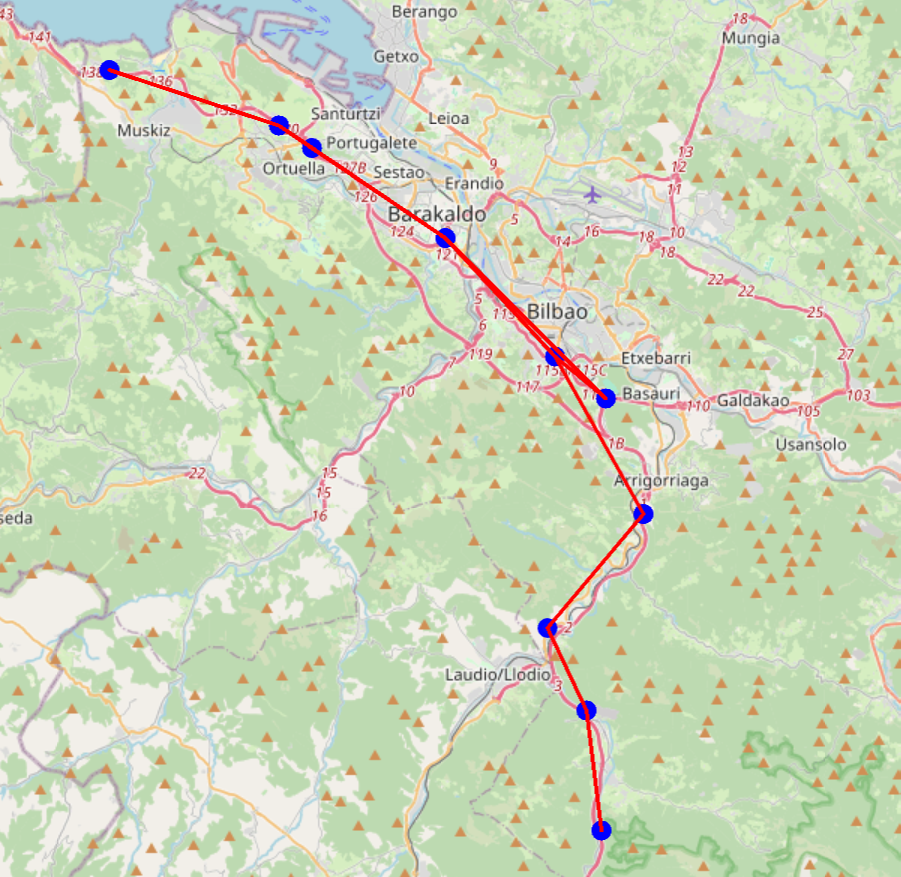
\includegraphics[width=0.5\linewidth]{includes/cap5/source_id_1_meters_mask.png}
	\caption{Distribución espacial de sensores para Gobierno Vasco (sourceId 1).}
	\label{fig:sensores_sid1}
\end{figure}

\begin{figure}[H]
	\centering
	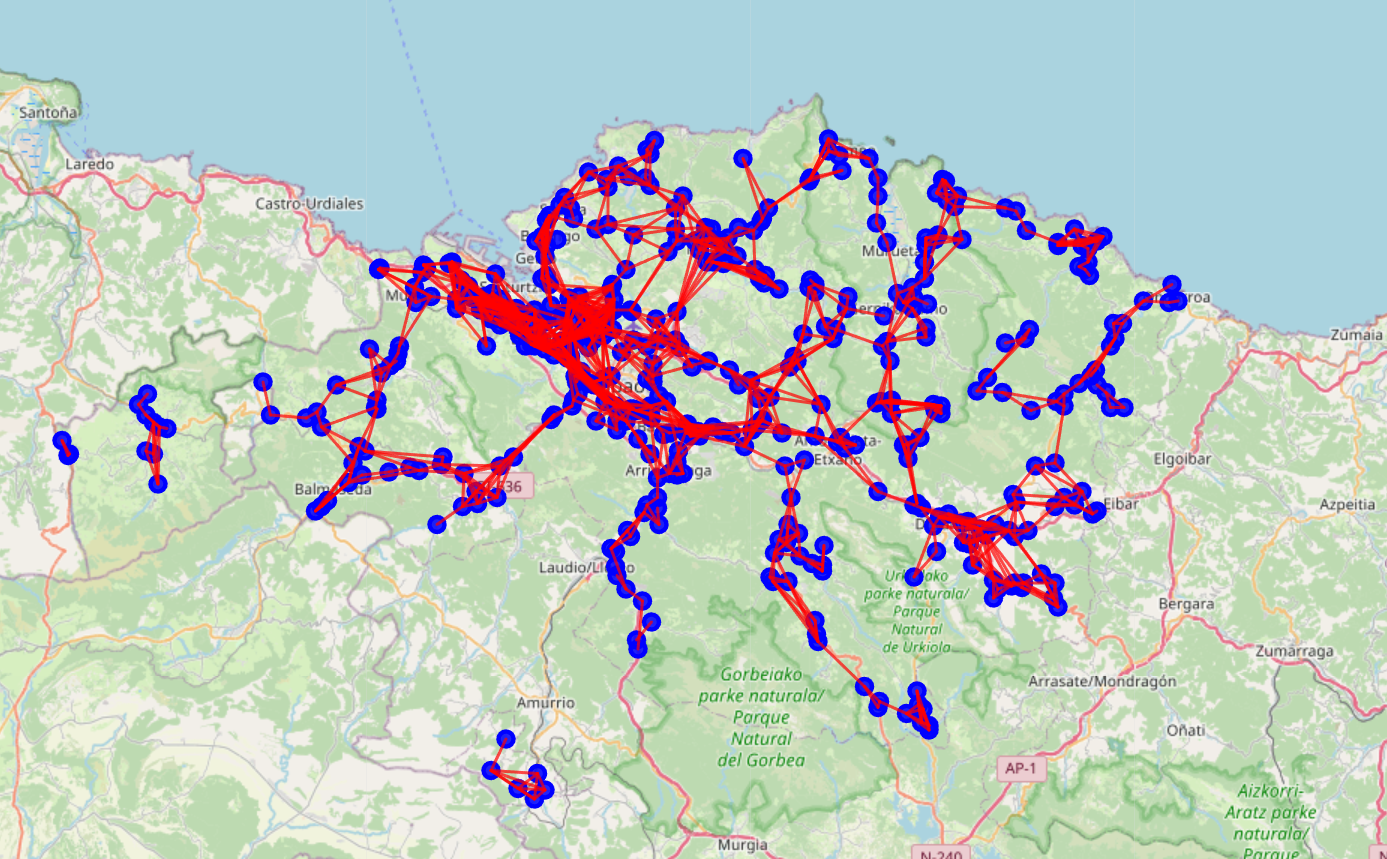
\includegraphics[width=0.7\linewidth]{includes/cap5/source_id_2_meters_mask.png}
	\caption{Distribución espacial de sensores para Diputación Foral de Bizkaia (sourceId 2).}
	\label{fig:sensores_sid2}
\end{figure}

\begin{figure}[H]
	\centering
	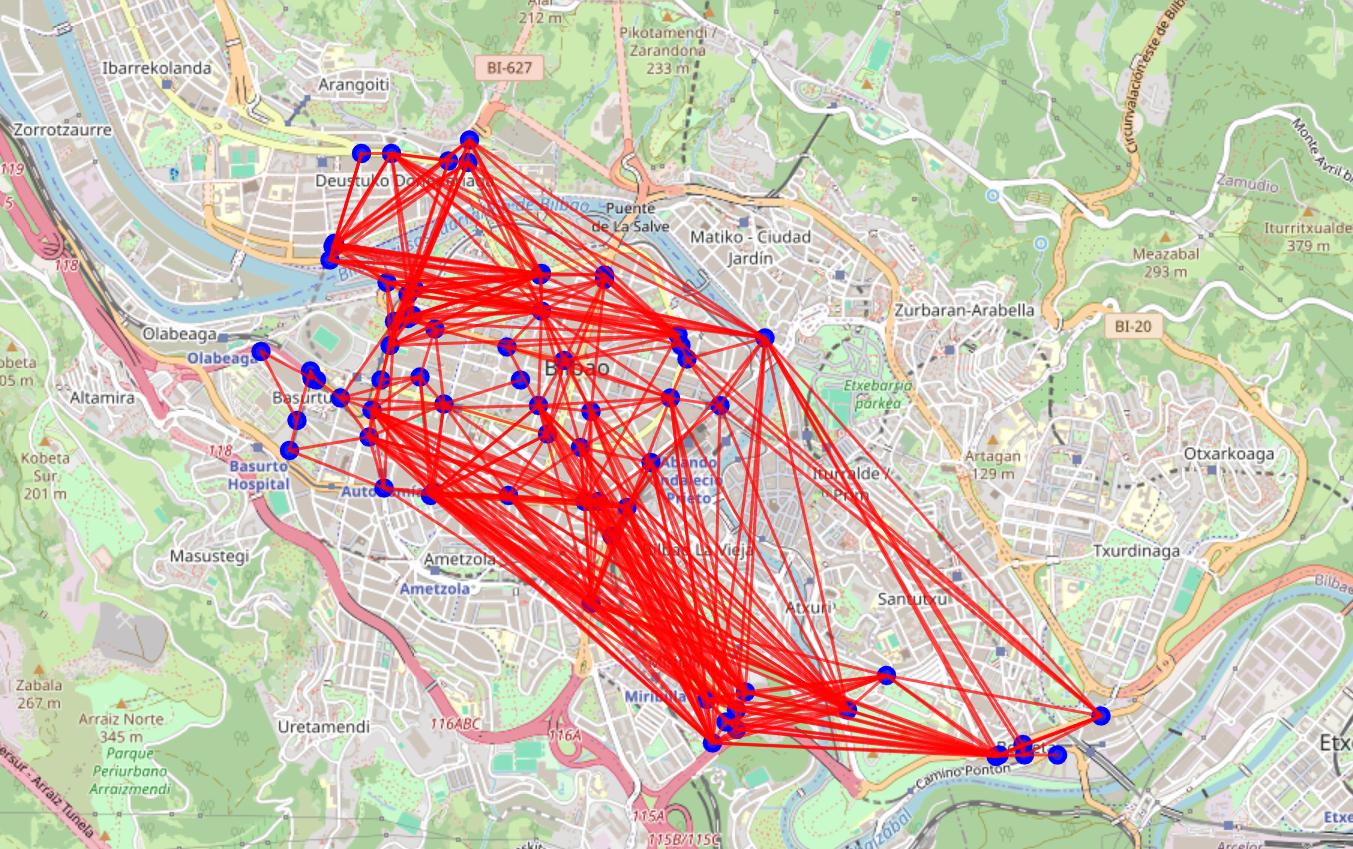
\includegraphics[width=0.7\linewidth]{includes/cap5/source_id_5_meters_mask.png}
	\caption{Distribución espacial de sensores para Ayuntamiento de Bilbao (sourceId 5).}
	\label{fig:sensores_sid5}
\end{figure}

A partir del grafo de sensores se puede derivar la matriz de adyacencia, que resulta clave para la aplicación de técnicas de enmascaramiento espacial y la explotación de correlaciones topológicas en los modelos de predicción.

\subsubsection*{Máscaras espaciales (solo para Trafficformer)}

Las máscaras espaciales permiten restringir el campo de atención del modelo, indicando qué sensores deben influenciarse entre sí durante el proceso de autoatención.

Se ha diseñado una arquitectura extensible de generación de máscaras, implementada en el paquete \texttt{mask}, con dos estrategias principales:

\begin{itemize}
	\item \texttt{BinarySpatialMaskStrategy}: enmascaramiento binario según distancia máxima.
	\item \texttt{OSMPathSpatialMaskStrategy}: estrategia principal utilizada, basada en conectividad vial real extraída de OpenStreetMap.
\end{itemize}

Estas máscaras se construyen en formato tensorial y se almacenan para su reutilización durante los entrenamientos posteriores.

\subsubsection*{Serialización y persistencia}

Todos los tensores generados (entradas, salidas, máscaras) se serializan en disco utilizando formatos como \texttt{.npz} y \texttt{.json}. Estos ficheros se almacenan de forma organizada por combinación de modelo y fuente de datos, y se respaldan en MinIO para garantizar su disponibilidad en posteriores ejecuciones.

Esta estrategia de persistencia permite:

\begin{itemize}
	\item Acelerar la experimentación al evitar preprocesado redundante.
	\item Asegurar reproducibilidad al asociar cada dataset a su configuración original.
	\item Compatibilidad con entornos remotos como AWS, donde se montan los datasets desde MinIO.
\end{itemize}

\subsection{Descripción de los modelos}
\label{sec:descripcion_modelos}

\begin{comment}
	- Explicación y justificación del modelo MLP y del modelo Trafficformer, apoyándose en tus propias docstrings y esquemas de arquitectura.
	- Tabla resumen de los principales hiperparámetros y variantes experimentadas.
\end{comment}

Durante el desarrollo de este trabajo se han implementado dos tipos de modelos de aprendizaje profundo para la predicción del flujo vehicular: un modelo base tipo perceptrón multicapa (MLP) y una arquitectura avanzada basada en Transformers denominada \texttt{Trafficformer}. Ambos modelos han sido implementados en PyTorch y diseñados para ajustarse al mismo pipeline de datos, permitiendo una comparación directa en términos de rendimiento y eficiencia.

\subsubsection*{Perceptrón Multicapa (MLP)}

El modelo \texttt{MLP}, implementado en el fichero \texttt{mlp\_enhanced.py}, actúa como modelo base para el conjunto de experimentos. Su arquitectura consiste en una serie de capas completamente conectadas (\texttt{Linear}), separadas por funciones de activación \texttt{ReLU}, normalización por lotes (\texttt{BatchNorm1d}) y capas de regularización \texttt{Dropout}.

Cada entrada al modelo consiste en un vector plano que concatena todas las variables relevantes para un conjunto de sensores a lo largo de una ventana temporal. No se incorpora ninguna estructura espacial, por lo que no hay noción de relaciones entre sensores.

El objetivo de este modelo es servir de referencia base o \textit{baseline}, tanto en términos de complejidad como de rendimiento, permitiendo comparar sus resultados con arquitecturas más sofisticadas.

En la Figura~\ref{fig:mlp_enhanced_vertical} 
 de capas.

\begin{figure}[H]
	\centering
	\begin{tikzpicture}[
		node distance=1.5cm,
		every node/.style={font=\small, align=center},
		box/.style={draw, rounded corners, minimum width=6.2cm, minimum height=1cm, fill=gray!5},
		arrow/.style={-Latex, thick}
		]
		% Nodes
		\node[box] (input) {[Input: batch, num\_meters, seq\_len, num\_features]};
		\node[box, below=of input] (flatten) {Flatten};
		\node[box, below=of flatten] (linear1) {Linear $\rightarrow$ hidden\_dim\\ReLU + BatchNorm + Dropout};
		\node[box, below=of linear1] (linear2) {Linear $\rightarrow$ hidden\_dim\\ReLU + BatchNorm + Dropout};
		\node[box, below=of linear2] (linear3) {Linear $\rightarrow$ 1};
		\node[box, below=of linear3] (reshape) {Reshape $\rightarrow$ batch $\times$ num\_meters};
		\node[box, below=of reshape] (output) {Output};
		
		% Arrows
		\draw[arrow] (input) -- (flatten);
		\draw[arrow] (flatten) -- (linear1);
		\draw[arrow] (linear1) -- (linear2);
		\draw[arrow] (linear2) -- (linear3);
		\draw[arrow] (linear3) -- (reshape);
		\draw[arrow] (reshape) -- (output);
	\end{tikzpicture}
	\caption{Esquema lógico del flujo de capas en el modelo \texttt{MLP}.}
	\label{fig:mlp_enhanced_vertical}
\end{figure}

El comportamiento del modelo está condicionado por varios parámetros configurables en su constructor:

\begin{itemize}
	\item \texttt{seq\_len}: longitud de la ventana temporal. Determina el número de pasos hacia atrás que observa el modelo por sensor. Ejemplo: 8, para las últimas 4 horas.
	\item \texttt{num\_features}: número de variables por paso temporal (meteorológicas, calendario, incidencias, etc.).
	\item \texttt{num\_meters}: cantidad de sensores simultáneos a predecir en una sola muestra.
	\item \texttt{hidden\_dim}: dimensión de las capas ocultas (\textbf{por defecto: 128}).
	\item \texttt{dropout}: probabilidad de desactivación aleatoria de neuronas durante el entrenamiento (\textbf{por defecto: 0.2}).
\end{itemize}

Estos parámetros permiten ajustar la capacidad del modelo a distintos tamaños de entrada y configuraciones experimentales, manteniendo una estructura modular y flexible.

\subsubsection*{Trafficformer}

El modelo \texttt{Trafficformer}, implementado en el fichero \texttt{trafficformer.py} e incluido en el \hyperref[anexo:codigo_trafficformer]{Anexo~E}, representa una evolución arquitectónica de los Transformers tradicionales adaptada al contexto específico de predicción de tráfico multivariable. A diferencia de las redes densas como el MLP, esta arquitectura se construye con el propósito de capturar de forma simultánea dependencias temporales a lo largo de una ventana de observación y relaciones espaciales entre sensores distribuidos por la red viaria.

Cada entrada al modelo es un tensor de cuatro dimensiones con forma \texttt{[batch, num\_nodes, seq\_len, num\_features]}, donde cada nodo (o sensor) contiene una secuencia temporal de medidas multivariantes. A este tensor se le aplica una codificación posicional sinusoidal, que permite al modelo distinguir la posición relativa de cada instante de tiempo dentro de la secuencia, ya que carece de una estructura recurrente que imponga orden implícito.

Seguidamente, cada nodo procesa localmente su secuencia temporal a través de un extractor de características basado en un perceptrón multicapa (\texttt{MLP}), dotado de capas \texttt{Linear}, activaciones \texttt{ReLU}, normalización \texttt{LayerNorm} y \texttt{Dropout}. Esto da lugar a un embedding por nodo que encapsula su evolución temporal reciente.

Una vez obtenidos estos embeddings, se procede a su procesamiento mediante un bloque encoder compuesto por múltiples capas Transformer apiladas. Estas capas aplican mecanismos de atención multi-cabezal (\texttt{MultiheadAttention}) modificados con una máscara espacial. Esta máscara restringe selectivamente la atención entre pares de sensores en función de su proximidad geográfica o conectividad vial, impidiendo que el modelo derive patrones entre sensores inconexos o lejanos. Esta técnica es especialmente útil en entornos urbanos donde la correlación entre sensores es local y estructural. El uso de máscaras basadas en grafos viales —derivados, por ejemplo, de OpenStreetMap— permite guiar la atención del modelo hacia relaciones físicamente plausibles.

Esta operación se ilustra esquemáticamente en la Figura~\ref{fig:attention_masking}, donde puede observarse cómo, para un nodo dado (por ejemplo, A), el mecanismo de atención restringe las relaciones posibles únicamente a aquellos nodos (como B o D) con los que mantiene una conexión válida según la máscara espacial predefinida. Los nodos no conectados —como C— quedan excluidos del proceso de atención mediante un enmascaramiento explícito. Este mecanismo refuerza la inductiva de la arquitectura, dotándola de una priorización estructural sobre la red vial que mejora la generalización y reduce la posibilidad de sobreajuste a correlaciones espurias.

\begin{figure}[H]
	\centering
	\begin{tikzpicture}[
		node distance=1.8cm,
		every node/.style={font=\small, align=center},
		box/.style={draw, rounded corners, minimum width=5.5cm, minimum height=1cm, fill=gray!5},
		arrow/.style={-Latex, thick}
		]
		% Nodes
		\node[box] (A) {Nodo A (sensor 1)};
		\node[box, below=of A] (att) {Atención multi-cabezal\\Q (query) $\leftarrow$ Nodo A\\K, V (keys, values) $\leftarrow$ Nodos B, C, D, E, ...};
		\node[box, below=of att] (mask) {Máscara espacial (M)\\[2pt]
			M[A][B] = 1 $\rightarrow$ se permite la atención\\
			M[A][C] = 0 $\rightarrow$ atención bloqueada\\
			M[A][D] = 1 $\rightarrow$ se permite la atención\\
			\textellipsis};
		\node[box, below=of mask] (rest) {Atención restringida por máscara};
		\node[box, below=of rest] (embed) {Embedding enriquecido del nodo A};
		
		% Arrows
		\draw[arrow] (A) -- (att);
		\draw[arrow] (att) -- (mask);
		\draw[arrow] (mask) -- (rest);
		\draw[arrow] (rest) -- (embed);
	\end{tikzpicture}
	\caption{Aplicación de la máscara espacial en el mecanismo de atención de \texttt{Trafficformer}.}
	\label{fig:attention_masking}
\end{figure}

Tras el bloque de atención se encuentra una red \texttt{FeedForward} con normalización y conexiones residuales, que complementa la capacidad de aprendizaje no lineal de la arquitectura. Finalmente, se aplica un bloque predictor por nodo, implementado como un MLP con estructura \texttt{Linear → LayerNorm → ReLU → Linear}, que emite la predicción del volumen de tráfico esperado en el próximo instante temporal.

El flujo completo de capas puede representarse de forma esquemática como sigue:

\begin{figure}[H]
	\centering
	\begin{tikzpicture}[
		node distance=1.8cm,
		every node/.style={font=\small, align=center},
		box/.style={draw, rounded corners, minimum width=6.2cm, minimum height=1cm, fill=gray!5},
		arrow/.style={-Latex, thick}
		]
		% Nodes
		\node[box] (input) {[Input: batch, num\_nodes, seq\_len, num\_features]};
		\node[box, below=of input] (posenc) {Positional Encoding};
		\node[box, below=of posenc] (mlp) {Temporal Feature Extractor\\MLP + LayerNorm + Dropout};
		\node[box, below=of mlp] (encoder) {Encoder Layer $\times$ N:\\Spatial Multi-Head Attention\\+ FeedForward + Residual};
		\node[box, below=of encoder] (pred) {Predictor MLP:\\Linear $\rightarrow$ LayerNorm $\rightarrow$ ReLU $\rightarrow$ Linear};
		\node[box, below=of pred] (output) {[Output: batch $\times$ num\_nodes]};
		
		% Arrows
		\draw[arrow] (input) -- (posenc);
		\draw[arrow] (posenc) -- (mlp);
		\draw[arrow] (mlp) -- (encoder);
		\draw[arrow] (encoder) -- (pred);
		\draw[arrow] (pred) -- (output);
	\end{tikzpicture}
	\caption{Esquema lógico del flujo de capas del modelo \texttt{Trafficformer}.}
	\label{fig:trafficformer_vertical}
\end{figure}

Cabe destacar que el modelo ha sido diseñado para ser altamente configurable, permitiendo ajustar su capacidad expresiva a distintos conjuntos de datos y requisitos computacionales. Entre los principales hiperparámetros se encuentran:

\begin{itemize}
	\item \texttt{seq\_len}: número de pasos temporales observados por nodo.
	\item \texttt{num\_features}: cantidad de variables por instante temporal.
	\item \texttt{embedding\_dim}: dimensión del vector que representa cada nodo tras el extractor de características.
	\item \texttt{num\_heads}: número de cabezales en el mecanismo de atención.
	\item \texttt{num\_layers}: número de capas encoder apiladas.
	\item \texttt{ff\_hidden\_dim}: tamaño intermedio en la red feedforward de cada encoder.
	\item \texttt{dropout}: tasa de desactivación de unidades durante el entrenamiento.
\end{itemize}

Esta flexibilidad, unida a su capacidad para integrar estructura espacial, convierte a \texttt{Trafficformer} en una solución avanzada para la predicción de tráfico en entornos reales complejos, como el caso de estudio abordado en este trabajo.

\subsection{Diseño experimental y combinaciones}
\label{sec:diseño_exp_combinaciones}

Para evaluar de forma rigurosa el rendimiento de las distintas arquitecturas propuestas, se ha diseñado un conjunto exhaustivo de experimentos que cubre diversas combinaciones de modelos, hiperparámetros y fuentes de datos. En concreto, el total de combinaciones generadas asciende a \textbf{120 experimentos}, resultado de combinar las 3 fuentes de datos preparadas (Gobierno Vasco, Diputación Foral de Bizkaia y Ayuntamiento de Bilbao), 2 arquitecturas principales (MLP y Trafficformer), y 20 configuraciones distintas de hiperparámetros. Cada uno de estos experimentos ha sido ejecutado de forma independiente y almacenado como notebook reproducible.

El diseño factorial considera dos modelos principales: \texttt{MLP} como base lineal y \texttt{Trafficformer} como modelo avanzado con atención espacial. A su vez, se han evaluado estas arquitecturas sobre tres conjuntos de datos procedentes de distintas fuentes institucionales, representadas por los identificadores \texttt{source\_id = 1, 2, 5}.

Cada modelo ha sido entrenado utilizando un conjunto diverso de combinaciones de hiperparámetros. En la Tabla~\ref{tab:experimentos_resumen} se presentan los valores explorados para cada parámetro, clasificados por arquitectura.

\begin{table}[H]
	\centering
	\small
	\caption{Configuraciones experimentales evaluadas}
	\label{tab:experimentos_resumen}
	\begin{tabularx}{\textwidth}{
			>{\centering\arraybackslash}c
			>{\centering\arraybackslash}c
			>{\centering\arraybackslash}c
			>{\centering\arraybackslash}c
			>{\centering\arraybackslash}c
			>{\centering\arraybackslash}c
			>{\centering\arraybackslash}c
			>{\centering\arraybackslash}c
			>{\centering\arraybackslash}X
	}
		\toprule
		\textbf{SID} & \textbf{M} & \textbf{SL} & \textbf{LR} & \textbf{BS} & \textbf{E/ESP} & \textbf{NH} & \textbf{ED} & \textbf{NL/FF} \\
		\midrule
		1 & MLP           & 4, 8 & 1e-3 / 5e-4 & 64 / 128 & 100 / 10  & -      & -        & - \\
		1 & Trafficformer & 4, 8 & 1e-3 / 5e-4 & 32 / 64  & 120 / 10  & 4 / 8  & 64 / 128 & 4/256 y 6/512 \\
		2 & MLP           & 4, 8 & 1e-3 / 1e-4 & 64 / 128 & 100 / 10  & -      & -        & - \\
		2 & Trafficformer & 4, 8 & 1e-3 / 1e-4 & 32 / 64  & 120 / 10  & 4 / 8  & 64 / 128 & 4/256 y 6/512 \\
		5 & MLP           & 4, 8 & 1e-3 / 5e-4 & 64 / 128 & 100 / 10  & -      & -        & - \\
		5 & Trafficformer & 4, 8 & 1e-3 / 5e-4 & 32 / 64  & 120 / =10 & 4 / 8  & 64 / 128 & 4/256 y 6/512 \\
		\bottomrule
	\end{tabularx}
\end{table}

A continuación, se detallan las combinaciones de hiperparámetros evaluadas en el conjunto de experimentos realizados. Cada uno de estos parámetros ha sido cuidadosamente seleccionado en base a recomendaciones de la literatura científica y su aplicabilidad práctica en modelos de predicción multivariada de series temporales, como se describe seguidamente:

\begin{itemize}
	\item \textbf{SourceId} (SID): La fuente de datos.
	\item \textbf{Modelo} (M): El modelo.
	\item \textbf{SEQ\_LEN} (SL): Los valores 4 y 8 permiten comparar el efecto de ventanas más cortas vs. más largas sobre la precisión y la capacidad de capturar patrones temporales. Es una práctica habitual en \textit{forecasting} experimentar con varias ventanas para encontrar el equilibrio entre capacidad de predicción y sobreajuste.
	\item \textbf{Learning Rate} (LR): 1e-3 es un valor estándar en \textit{deep learning} y recomendado en el propio artículo de Trafficformer~\cite{trafficformer}, pero se elige 5e-4 para realizar el experimento. En el articulo también se cita el empleo de la estrategia ReduceLROnPlateau \cite{ruder2017overviewgradientdescentoptimization}, estrategia que permite reducir el learning rate hasta un umbral en función de la selección de una métrica. Pese a que dicha estrategia está disponible en Pytorch \cite{pytorchReduceLrOnPLateau} se decidió no emplearla por reducir la complejidad del experimento.
	\item \textbf{Batch Size} (BS): Se experimenta con 64 y 128 para MLP, y con 32 y 64 para Trafficformer. Un \textit{batch size} menor en Trafficformer permite reducir el uso de memoria y mejora la generalización en modelos más profundos.
	\item \textbf{Epochs / Early Stopping, Patience} (E/ESP): Se ha limitado el entrenamiento a 100--120 épocas, con un mecanismo de \textit{early stopping} con paciencia de 10 épocas. Esta configuración evita el sobreentrenamiento sin necesidad de vigilancia manual.
	\item \textbf{NUM\_HEADS} (NH) y \textbf{EMBEDDING\_DIM} (ED): Las combinaciones evaluadas (4/64 y 8/128) reflejan el equilibrio entre capacidad representacional y coste computacional. Un mayor número de cabezas puede capturar relaciones más complejas entre sensores.
	\item \textbf{NUM\_LAYERS} (NL) y \textbf{FF\_HIDDEN\_DIM} (FF): Se han probado configuraciones de 4 capas con 256 dimensiones ocultas y 6 capas con 512. Estos valores están alineados con los recomendados en el artículo original y en benchmarks del estado del arte.
\end{itemize}

Cada experimento fue registrado y monitorizado utilizando la plataforma \texttt{Weights \& Biases}, lo que permitió realizar un análisis sistemático posterior y facilitar la selección de los mejores modelos por fuente de datos y arquitectura. Para facilitar la reproducibilidad y la trazabilidad de los resultados, todos los notebooks están numerados de forma consistente e incluyen visualizaciones, métricas y configuración exacta de entrenamiento.

En el \hyperref[anexo:combinaciones_exp]{Anexo~F} se pueden consultar las diferentes combinaciones experimentales propuestas.

\subsection{Proceso de entrenamiento y selección de mejores modelos}
\label{sec:entrenamiento_mej_modelos}

El proceso de entrenamiento de los modelos se ha realizado bajo un entorno controlado y reproducible, siguiendo las mejores prácticas en experimentación con redes neuronales. Para ello, se han desarrollado cuadernos Jupyter donde se define de manera explícita cada paso del ciclo experimental: carga de datos, configuración del entorno, definición del modelo, entrenamiento, evaluación y registro de resultados.

\subsubsection*{Configuración y reproducibilidad}  
El entorno de trabajo se inicializa con la carga de variables de entorno desde ficheros \texttt{.env}, estableciendo parámetros como la conexión a la base de datos MongoDB, claves de autenticación para \textit{Weights \& Biases} (Wandb), y valores por defecto de hiperparámetros como \texttt{batch size}, \texttt{learning rate}, \texttt{dropout} o \texttt{hidden dimensions}. Se fija una semilla aleatoria global para asegurar la reproducibilidad entre ejecuciones, controlando el estado de generación de números aleatorios tanto de \texttt{NumPy}, \texttt{Python} como de \texttt{PyTorch} (CPU y GPU).

\subsubsection*{Carga del dataset y preparación}  
Se emplea una clase personalizada \texttt{TrafficDataset}, diseñada para conectarse directamente a la base de datos y construir un conjunto de muestras a partir de una ventana temporal configurable (\texttt{SEQ\_LEN}). El conjunto de datos incluye tanto variables numéricas escaladas (\texttt{StandardScaler}), como categóricas codificadas (\texttt{OneHotEncoder}) y booleanas convertidas a \texttt{float} con valores binarios. Las variables faltantes se imputan de forma segura mediante media (\texttt{mean}) para variables continuas y con cero para booleanos. La división de datos se realiza de forma estratificada y reproducible en tres subconjuntos: entrenamiento (70\%), validación (20\%) y test (10\%).

\subsubsection*{Máscara espacial y visualización}  
Para los modelos tipo Transformer, se genera una máscara espacial binaria que codifica qué sensores de tráfico pueden atenderse entre sí, basada en criterios geográficos extraídos desde OpenStreetMap (vía GraphML). Esta máscara se emplea durante el mecanismo de atención multi-cabezal. Se valida la consistencia entre los sensores del dataset y la máscara, y se genera una visualización interactiva de la red de sensores y sus enlaces espaciales, posteriormente registrada como artefacto en Wandb.

\subsubsection*{Inicialización del modelo y optimización}  
El modelo se instancia según el tipo elegido (\texttt{TrafficMLPEnhanced} o \texttt{Trafficformer}), utilizando parámetros definidos al inicio del experimento. El criterio de pérdida utilizado es el error cuadrático medio (\texttt{MSELoss}), y el optimizador elegido es \texttt{AdamW}, con tasa de aprendizaje inicial y \texttt{weight decay} ajustables. El modelo y el criterio son registrados en Wandb, junto con los hiperparámetros y la configuración del experimento.

\subsubsection*{Entrenamiento supervisado y \textit{early stopping}}  
El bucle de entrenamiento se ejecuta durante un máximo de 100--120 épocas, con activación de un mecanismo de \textit{early stopping} basado en la pérdida de validación con una paciencia de 10 épocas. Por cada época, se computan las métricas \texttt{MSE}, \texttt{MAE}, \texttt{RMSE}, \texttt{MAPE} y \texttt{R\textsuperscript{2}} para los tres subconjuntos (train, val, test). Además, se monitoriza el uso de memoria RAM y GPU, el tiempo de inferencia por muestra y la duración total por época.

En cada iteración se guardan:

\begin{itemize}
	\item Un \textit{checkpoint} del estado actual del modelo, optimizador y estados aleatorios.
	\item La historia de métricas en un fichero CSV.
	\item El mejor modelo según pérdida de validación.
\end{itemize}

\subsubsection*{Evaluación y seguimiento}  
Al finalizar el entrenamiento, se guarda el modelo final, se registra el tiempo total del proceso y se finaliza la sesión de WandB. Además, se generan gráficas para cada métrica de evaluación, comparando la evolución entre entrenamiento y validación. La mejor época se corresponde con la mínima pérdida de validación y se resalta en cada gráfica. Estas curvas permiten detectar patrones de sobreentrenamiento, estancamiento o mejoras progresivas en el aprendizaje.

\begin{figure}[H]
	\centering
	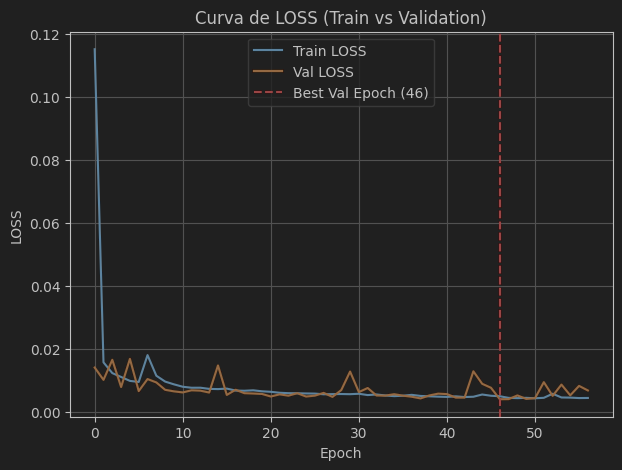
\includegraphics[width=0.5\textwidth]{includes/cap5/loss_curve_example.png}
	\caption{Curvas de evolución de pérdida para entrenamiento y validación, con indicación de la mejor época.}
	\label{fig:loss_curve_example}
\end{figure}

\subsubsection*{Registro de resultados y comparación}  
Cada experimento queda documentado y reproducible mediante artefactos almacenados en el sistema de ficheros y sincronizados con la plataforma \textit{Weights \& Biases}. Esto incluye mapas de sensores, configuración exacta, métricas por época, curvas de entrenamiento y modelos entrenados. El historial completo permite comparar el rendimiento de diferentes combinaciones de hiperparámetros, tanto a nivel visual como mediante agregación tabular.
